\chapter{Discussion and conclusions}
\todo{Add content, cf. thesis structure proposal}

BepuPhysics2 proved to be an excellent choice for a video game physics engine.
Our tests, such as the one depicted in \autoref{fig:bepu-lots-of-stuff} show that it's able to handle large workloads.
In this particular test, we spawned 100 bots, each firing projectiles at the player.
Despite this workload on the physics engine, the application still managed to work without lags.
\begin{figure}[h] % I can't emphasize how much I love this picture
    \centering
    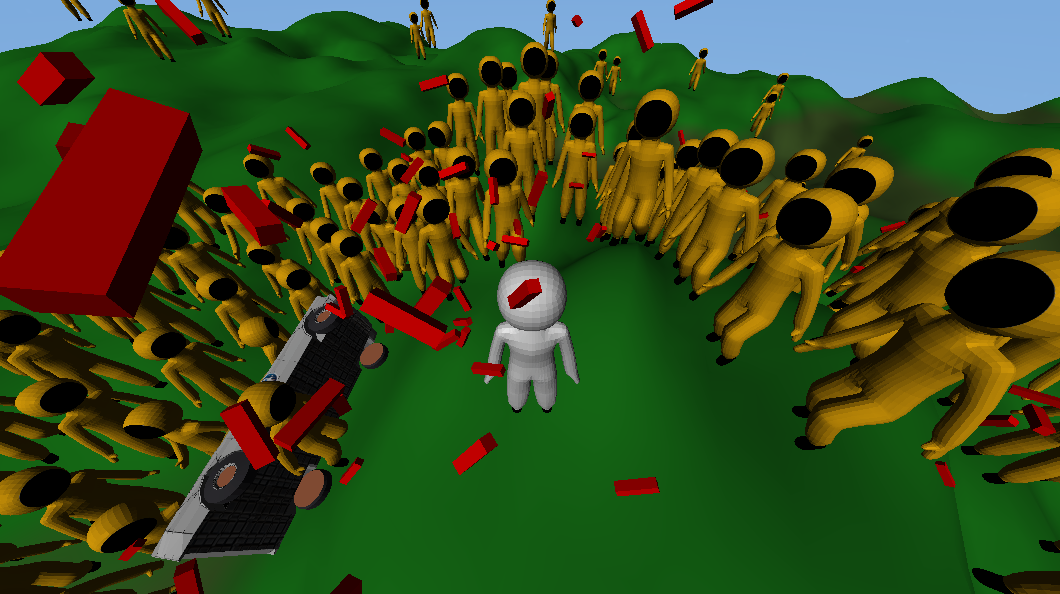
\includegraphics[width=0.8\textwidth]{chapters/discussion_and_conclusions/resources/lots-of-stuff.png}
    \caption{BepuPhysics library taken to the extremee}
    \label{fig:bepu-lots-of-stuff}
\end{figure}

